\documentclass[14pt]{extbook}
\usepackage{multicol, enumerate, enumitem, hyperref, color, soul, setspace, parskip, fancyhdr} %General Packages
\usepackage{amssymb, amsthm, amsmath, latexsym, units, mathtools} %Math Packages
\everymath{\displaystyle} %All math in Display Style
% Packages with additional options
\usepackage[headsep=0.5cm,headheight=12pt, left=1 in,right= 1 in,top= 1 in,bottom= 1 in]{geometry}
\usepackage[usenames,dvipsnames]{xcolor}
\usepackage{dashrule}  % Package to use the command below to create lines between items
\newcommand{\litem}[1]{\item#1\hspace*{-1cm}\rule{\textwidth}{0.4pt}}
\pagestyle{fancy}
\lhead{Progress Quiz 9}
\chead{}
\rhead{Version A}
\lfoot{9541-5764}
\cfoot{}
\rfoot{Summer C 2021}
\begin{document}

\begin{enumerate}
\litem{
For the graph below, evaluate the limit: $ \displaystyle \lim_{x \rightarrow 3} f(x)$.
\begin{center}
    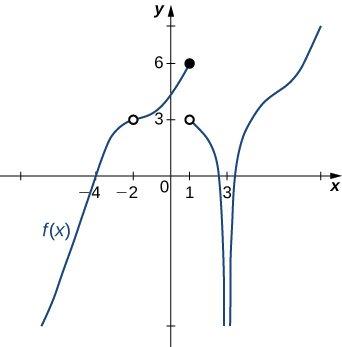
\includegraphics[width=0.5\textwidth]{../Figures/evaluateLimitGraphicallyA.png}
\end{center}
\begin{enumerate}[label=\Alph*.]
\item \( -\infty \)
\item \( -2 \)
\item \( 1 \)
\item \( \text{The limit does not exist} \)
\item \( \text{None of the above} \)

\end{enumerate} }
\litem{
Evaluate the one-sided limit of the function $f(x)$ below, if possible.\[ \lim_{x \rightarrow 2^-} \frac{1}{(x+2)^3}+9 \]\begin{enumerate}[label=\Alph*.]
\item \( f(2) \)
\item \( \infty \)
\item \( -\infty \)
\item \( \text{The limit does not exist} \)
\item \( \text{None of the above} \)

\end{enumerate} }
\litem{
For the graph below, find the value(s) $a$ that makes the statement true: $ \displaystyle \lim_{x \rightarrow a} f(x)$ does not exist.
\begin{center}
    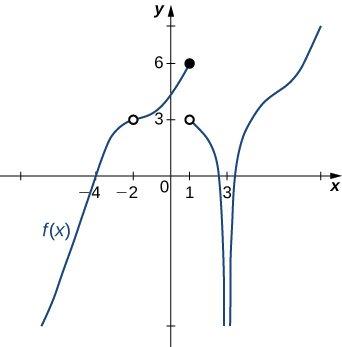
\includegraphics[width=0.5\textwidth]{../Figures/evaluateLimitGraphicallyCopyA.png}
\end{center}
\begin{enumerate}[label=\Alph*.]
\item \( 1 \)
\item \( 3 \)
\item \( -2 \)
\item \( \text{Multiple } a \text{ make the statement true}. \)
\item \( \text{No } a \text{ make the statement true}. \)

\end{enumerate} }
\litem{
Based on the information below, which of the following statements is always true?
\begin{center}
    \textit{ $f(x)$ approaches $11.29$ as $x$ approaches $\infty$. }
\end{center}
\begin{enumerate}[label=\Alph*.]
\item \( f(x) \text{ is close to or exactly } 11.29 \text{ when } x \text{ is large enough}. \)
\item \( x \text{ is undefined when } f(x) \text{ is large enough}. \)
\item \( f(x) \text{ is close to or exactly } \infty \text{ when } x \text{ is large enough}. \)
\item \( f(x) \text{ is undefined when } x \text{ is large enough}. \)
\item \( \text{None of the above are always true.} \)

\end{enumerate} }
\litem{
To estimate the one-sided limit of the function below as $x$ approaches 9 from the right, which of the following sets of numbers should you use?\[ \frac{\frac{9}{x} - 1}{x - 9} \]\begin{enumerate}[label=\Alph*.]
\item \( \{ 8.9000, 8.9900, 9.0100, 9.1000 \} \)
\item \( \{ 8.9000, 8.9900, 8.9990, 8.9999 \} \)
\item \( \{ 9.0000, 9.1000, 9.0100, 9.0010 \} \)
\item \( \{ 9.1000, 9.0100, 9.0010, 9.0001 \} \)
\item \( \{ 9.0000, 8.9000, 8.9900, 8.9990 \} \)

\end{enumerate} }
\litem{
Evaluate the limit below, if possible.\[ \lim_{x \rightarrow 3} \frac{\sqrt{7x - 5} - 4}{8x - 24} \]\begin{enumerate}[label=\Alph*.]
\item \( 0.125 \)
\item \( \infty \)
\item \( 0.331 \)
\item \( 0.016 \)
\item \( \text{None of the above} \)

\end{enumerate} }
\litem{
Evaluate the limit below, if possible.\[ \lim_{x \rightarrow 7} \frac{\sqrt{6x - 26} - 4}{9x - 63} \]\begin{enumerate}[label=\Alph*.]
\item \( 0.125 \)
\item \( 0.272 \)
\item \( \infty \)
\item \( 0.014 \)
\item \( \text{None of the above} \)

\end{enumerate} }
\litem{
Based on the information below, which of the following statements is always true?
\begin{center}
    \textit{ $f(x)$ approaches $6.935$ as $x$ approaches $\infty$. }
\end{center}
\begin{enumerate}[label=\Alph*.]
\item \( f(x) \text{ is close to or exactly } 6.935 \text{ when } x \text{ is large enough}. \)
\item \( f(x) \text{ is close to or exactly } \infty \text{ when } x \text{ is large enough}. \)
\item \( f(x) \text{ is undefined when } x \text{ is large enough}. \)
\item \( x \text{ is undefined when } f(x) \text{ is large enough}. \)
\item \( \text{None of the above are always true.} \)

\end{enumerate} }
\litem{
Evaluate the one-sided limit of the function $f(x)$ below, if possible.\[ \lim_{x \rightarrow -6^-} \frac{-5}{(x-6)^8}+2 \]\begin{enumerate}[label=\Alph*.]
\item \( f(-6) \)
\item \( -\infty \)
\item \( \infty \)
\item \( \text{The limit does not exist} \)
\item \( \text{None of the above} \)

\end{enumerate} }
\litem{
To estimate the one-sided limit of the function below as $x$ approaches 6 from the right, which of the following sets of numbers should you use?\[ \frac{\frac{6}{x} - 1}{x - 6} \]\begin{enumerate}[label=\Alph*.]
\item \( \{ 6.0000, 6.1000, 6.0100, 6.0010 \} \)
\item \( \{ 5.9000, 5.9900, 5.9990, 5.9999 \} \)
\item \( \{ 6.1000, 6.0100, 6.0010, 6.0001 \} \)
\item \( \{ 5.9000, 5.9900, 6.0100, 6.1000 \} \)
\item \( \{ 6.0000, 5.9000, 5.9900, 5.9990 \} \)

\end{enumerate} }
\end{enumerate}

\end{document}